% SC1007 — Chapter 5: Heaps & Priority Queues
% No \documentclass — included by modules/SC1007/main.tex (book class).
\chapter{Heaps \& Priority Queues}
\label{ch:heaps-priority}

\begin{quote}
\emph{``The smallest is always on top.''} --- A heap trades total order for instant access to the extremum.
\end{quote}

\noindent\textbf{Prerequisites:} Ch.~3 (trees), Ch.~1 (arrays). Heap is an array-embedded tree giving $O(\log n)$ priority-queue ops and $O(n\log n)$ sorting.

\section*{Learning Outcomes}
After this chapter you will be able to:
\begin{enumerate}[label=(L\arabic*)]
    \item state the heap invariant and map heap indices to tree positions;
    \item implement \texttt{push}, \texttt{pop}, \texttt{heapify} with sift-up/down;
    \item build a heap in $O(n)$ via bottom-up heapify and prove it;
    \item use priority queues for scheduling and preview heap sort / Dijkstra.
\end{enumerate}

% ============================================================
\section{The Heap Invariant}
\label{sec:heap-invariant}
A (min-)heap is a \emph{complete} binary tree where every node $\le$ its children. The minimum is at the root. Completeness means all levels are full except possibly the last, filled left-to-right --- so the tree maps perfectly to an array.

\begin{equation}
\text{For } i \text{ (1-indexed): } \text{parent}(i)=\lfloor i/2\rfloor,\;
\text{left}(i)=2i,\; \text{right}(i)=2i+1.
\label{eq:heap-index}
\end{equation}
With 0-indexed arrays: parent $(i-1)/2$, children $2i+1,2i+2$.

\begin{figure}[h]
\centering
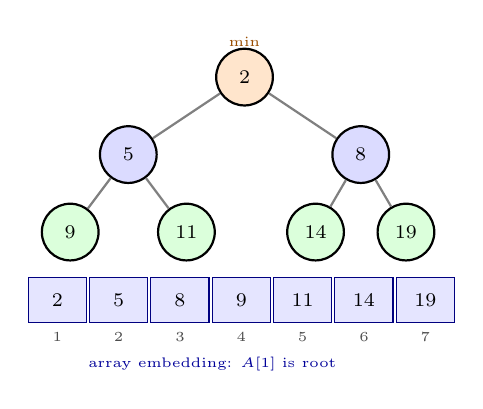
\begin{tikzpicture}[scale=0.82, every node/.style={font=\scriptsize},
  hnode/.style={circle, draw, thick, fill=blue!14, minimum size=0.72cm},
  edge/.style={thick, black!50}]
  % Tree
  \node[hnode, fill=orange!20] (1) at (3,2.6) {2};
  \node[hnode] (2) at (1.2,1.4) {5};
  \node[hnode] (3) at (4.8,1.4) {8};
  \node[hnode, fill=green!14] (4) at (0.3,0.2) {9};
  \node[hnode, fill=green!14] (5) at (2.1,0.2) {11};
  \node[hnode, fill=green!14] (6) at (4.1,0.2) {14};
  \node[hnode, fill=green!14] (7) at (5.5,0.2) {19};
  \draw[edge] (1)--(2); \draw[edge] (1)--(3); \draw[edge] (2)--(4); \draw[edge] (2)--(5);
  \draw[edge] (3)--(6); \draw[edge] (3)--(7);
  \node[font=\tiny, orange!60!black] at (3,3.15) {min};
  % Array below
  \begin{scope}[yshift=-1.2cm, xshift=-0.8cm]
    \foreach \i/\v in {1/2,2/5,3/8,4/9,5/11,6/14,7/19} {
      \draw[fill=blue!10, draw=blue!50!black] (\i*0.95-0.5,0) rectangle ++(0.90,0.70);
      \node at (\i*0.95-0.05,0.35) {\v};
      \node[font=\tiny, gray!60!black] at (\i*0.95-0.05,-0.22) {\i};
    }
    \node[font=\tiny, blue!60!black] at (3.3,-0.65) {array embedding: $A[1]$ is root};
  \end{scope}
\end{tikzpicture}
\caption{Min-heap as tree (top) and array (bottom). Every parent $\le$ children; completeness gives $O(1)$ index arithmetic.}
\label{fig:heap-array}
\end{figure}

Not a BST: heap only orders parent vs.\ child, not left vs.\ right. Inorder is not sorted.

% ============================================================
\section{Priority-Queue Operations}
\label{sec:pq-ops}

\begin{figure}[h]
\centering
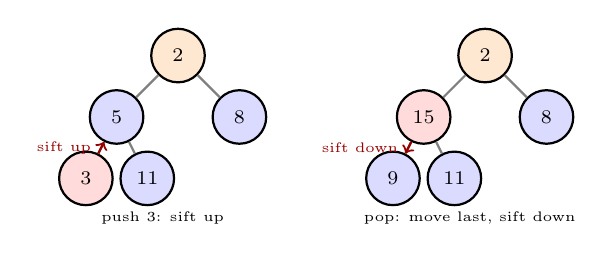
\begin{tikzpicture}[scale=0.78, every node/.style={font=\scriptsize},
  hnode/.style={circle, draw, thick, fill=blue!14, minimum size=0.68cm},
  edge/.style={thick, black!50}]
  % Sift-up illustration
  \begin{scope}
    \node[hnode, fill=orange!18] (a1) at (1.5,1.8) {2};
    \node[hnode] (a2) at (0.5,0.8) {5};
    \node[hnode] (a3) at (2.5,0.8) {8};
    \node[hnode, fill=red!14] (a4) at (0.0, -0.2) {3};
    \node[hnode] (a5) at (1.0,-0.2) {11};
    \draw[edge] (a1)--(a2); \draw[edge] (a1)--(a3); \draw[edge] (a2)--(a4); \draw[edge] (a2)--(a5);
    \draw[->, red!60!black, thick] (a4) -- (a2) node[midway, left, font=\tiny] {sift up};
    \node at (1.25,-0.85) {\tiny push 3: sift up};
  \end{scope}
  \begin{scope}[xshift=5cm]
    \node[hnode, fill=orange!18] (b1) at (1.5,1.8) {2};
    \node[hnode, fill=red!14] (b2) at (0.5,0.8) {15};
    \node[hnode] (b3) at (2.5,0.8) {8};
    \node[hnode] (b4) at (0.0,-0.2) {9};
    \node[hnode] (b5) at (1.0,-0.2) {11};
    \draw[edge] (b1)--(b2); \draw[edge] (b1)--(b3); \draw[edge] (b2)--(b4); \draw[edge] (b2)--(b5);
    \draw[->, red!60!black, thick] (b2) -- (b4) node[midway, left, font=\tiny] {sift down};
    \node at (1.25,-0.85) {\tiny pop: move last, sift down};
  \end{scope}
\end{tikzpicture}
\caption{Sift-up after insertion (left) and sift-down after extraction (right). Each follows one root-to-leaf path: $O(\log n)$.}
\label{fig:sift}
\end{figure}

\begin{lstlisting}[language=Python]
import heapq  # Python min-heap (0-indexed)

def push(heap, x):
    heap.append(x)
    i = len(heap) - 1
    while i > 0:
        p = (i - 1) // 2
        if heap[p] <= heap[i]: break
        heap[p], heap[i] = heap[i], heap[p]
        i = p  # sift up -- O(log n)

def pop(heap):
    if len(heap) == 1: return heap.pop()
    top = heap[0]
    heap[0] = heap.pop()  # move last to root
    i = 0
    while True:  # sift down -- O(log n)
        l, r = 2*i+1, 2*i+2
        smallest = i
        if l < len(heap) and heap[l] < heap[smallest]: smallest = l
        if r < len(heap) and heap[r] < heap[smallest]: smallest = r
        if smallest == i: break
        heap[i], heap[smallest] = heap[smallest], heap[i]
        i = smallest
    return top
\end{lstlisting}

\texttt{peek} $=$ \texttt{heap[0]} in $O(1)$. \texttt{decreaseKey} at index $i$ sifts up in $O(\log n)$.

% ============================================================
\section{Building a Heap in $O(n)$}
\label{sec:build-heap}
Naively pushing $n$ items costs $O(n\log n)$. Bottom-up \texttt{heapify} does it in $O(n)$: process nodes from $n/2$ down to $1$, sifting each down. Shorter subtrees dominate the sum.

\begin{align}
\sum_{h=0}^{\lfloor\log n\rfloor} \lceil n/2^{h+1}\rceil\cdot O(h)
= O\!\left(n\sum_{h\ge0} h/2^{h}\right) = O(n),
\label{eq:build-heap}
\end{align}
since $\sum h/2^{h}=2$.

\begin{figure}[h]
\centering
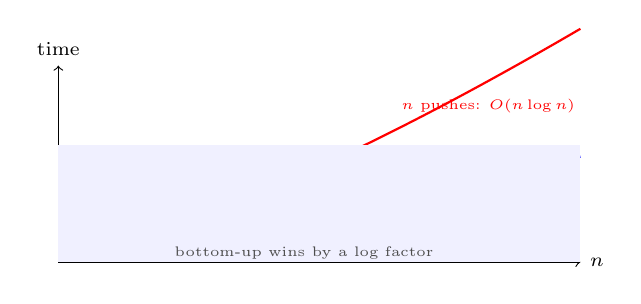
\begin{tikzpicture}[scale=0.78, every node/.style={font=\scriptsize}]
  \draw[->] (0,0) -- (8.5,0) node[right] {$n$};
  \draw[->] (0,0) -- (0,3.2) node[above] {time};
  \draw[red, thick] plot[domain=0.3:8.5, smooth] (\x,{0.25+0.45*\x*ln(\x+1)/ln(2)/3.5});
  \node[red, font=\tiny] at (7.0,2.55) {$n$ pushes: $O(n\log n)$};
  \draw[blue, thick] plot[domain=0.3:8.5, smooth] (\x,{0.25+0.38*\x/2.2});
  \node[blue, font=\tiny] at (7.0,1.55) {heapify: $O(n)$};
  \fill[blue!6] (0,0) rectangle (8.5,1.9);
  \node[font=\tiny, gray!60!black] at (4,0.15) {bottom-up wins by a log factor};
\end{tikzpicture}
\caption{Heap construction: repeated push vs.\ bottom-up heapify.}
\label{fig:build-heap-cost}
\end{figure}

\begin{lstlisting}[language=C++]
// C++ STL priority queue (max-heap by default)
#include <queue>
std::priority_queue<int> pq;          // max-heap
pq.push(5); pq.push(2); pq.push(8);
int top = pq.top();  // 8
pq.pop();            // removes 8

// min-heap variant
std::priority_queue<int, std::vector<int>, std::greater<int>> minpq;
\end{lstlisting}

% ============================================================
\section{Applications Preview}
Heap sort: build heap $O(n)$, repeatedly pop min $O(n\log n)$ in-place. Dijkstra's algorithm (Ch.~7) uses a min-heap to extract the closest unsettled vertex in $O((n+m)\log n)$.

% ============================================================

% --- Additional: Heap variants ---
\section{Variants \& Analysis Details}
\label{sec:heap-variants}
\textbf{Max-heap vs.\ min-heap.} Flip comparison. Max-heap gives descending sort by repeated extraction; min-heap is natural for Dijkstra (Ch.~7).

\textbf{$d$-ary heap.} Each node has $d$ children; height $\log_{d}n$, sift-down compares $d$ children. Choose $d$ to trade off sift-up vs.\ sift-down for the workload.

\textbf{Decrease-key.} After lowering $A[i]$, sift up restores heap in $O(\log n)$ --- essential for Dijkstra and Prim.

\begin{lstlisting}[language=Python]
# heapq is min-heap; max-heap via negation
import heapq
max_heap = []
for x in [5,2,8,1]: heapq.heappush(max_heap, -x)
top = -heapq.heappop(max_heap)  # 8

# Decrease-key at index i (min-heap)
def decrease_key(heap, i, new_val):
    assert new_val <= heap[i]
    heap[i] = new_val
    while i > 0:
        p = (i-1)//2
        if heap[p] <= heap[i]: break
        heap[p], heap[i] = heap[i], heap[p]
        i = p
\end{lstlisting}

\section{Chapter Notes}
CLRS Ch.~6, Weiss Ch.~6. Heap as priority queue vs.\ sorted array vs.\ balanced BST trade-offs.

% ============================================================
\section{Exercises}
\label{sec:ch05-exercises}
\begin{enumerate}[label=E5.\arabic*, leftmargin=*, itemsep=0.7em]
    \item \textbf{Heap ops.} Insert $4,8,2,9,5,11,14,3$ into empty min-heap (array order). Show array after each insert and after two \texttt{pop}s.
    \item \textbf{Build-heap proof.} Prove Eq.~\eqref{eq:build-heap} sums to $O(n)$ by bounding $\sum h/2^{h}$. Why does sifting from $n/2$ down to $1$ suffice (leaves need no work)?
    \item \textbf{Heap vs.\ BST.} Give an array that is a valid min-heap but whose inorder is not sorted. Explain why heap search for arbitrary key is $\Theta(n)$.
    \item \textbf{$k$-way merge.} Merge $k$ sorted arrays of total size $n$ using a heap in $O(n\log k)$. Prove your bound and show it beats pairwise merging.
    \item \textbf{Heap sort in-place.} Describe in-place heap sort on array $A[1..n]$ (build max-heap, swap max to end, shrink). Analyse space $O(1)$ auxiliary and stability.
\end{enumerate}
% End of Chapter 5
